\documentclass{article}

% Packages
\usepackage{tcolorbox}
\usepackage{amsmath}
\usepackage{amssymb}
\usepackage{caption}

% Global Settings
\captionsetup[table]{skip=10pt}

\begin{document}

\begin{titlepage}
    \begin{center}
        \LARGE{\textbf{CAB203 Discrete Structures}} \\[0.2in]
        \LARGE{Lecture Notes} \\[0.1in]
        \large{Jack Girard 2023}
    \end{center}
\end{titlepage}

\newpage

\tableofcontents
\newpage

\section{What is Mathematics?}
\subsection{What is Mathematics?}
\subsubsection{Abstraction}
Abstraction can be used to simplify a problem by ignoring all the information that is not needed.
They capture the relevant properties of a situation, and the relationships between them.
Those properties can then be used to work out the solution.
\begin{itemize}
    \item You have \(x\) apples
    \item You have \(y\) friends
    \item Are there enough apples for all your friends?
\end{itemize}
The usual abstraction for problems involving counting is \emph{natural numbers} (non-negative integers).
By abstracting away irrelevant properties such as size, shape, colour etc. the problem can be simplified to:
\[x \geq y?\]
Limitations of abstractions can include:
\begin{itemize}
    \item Not enough information
    \item Too much information
    \item Incorrect information
\end{itemize}
%
\subsubsection{Mathematical Theories}
An abstraction without reference to a particular problem is called a \emph{mathematical theory}, usually consisting of:
\begin{itemize}
    \item Mathematical objects (numbers, operations, etc.)
    \item Axioms (statements about how objects relate to each other)
\end{itemize}
%
\newpage
\subsubsection{Axioms}
Some examples of axioms for the natural numbers include:
\begin{enumerate}
    \item 0 is a natural number
    \item \(x = x\)
    \item if \(x = y\) then \(y = x\)
    \item if \(x = y\) and \(y = z\) then \(x = z\)
    \item if \(x = w\) then \(w\) is a natural number
    \item \(S(x)\) is a natural number
    \item if \(S(x) = S(y)\) then \(x = y\)
    \item \(S(x) = 0\) is always false
\end{enumerate}
Axioms can be combined to create new true statements.
For example, axiom 6 in the list above states \(S(x)\) is a natural number,
so by combining it with itself it can be deduced that \(S(S(x))\) is also a natural number.
\begin{tcolorbox}[title=Note]
    \begin{center}
        \(S\) refers to the \emph{successor function} that increments a natural number.
        \[S(x) = x + 1\]
    \end{center}
\end{tcolorbox}
%
\subsubsection{Mathematical Objects}
Mathematical objects are abstract objects that can correspond to concrete objects.
They can only be defined in how they relate to other objects - this is done through axioms.
Formally, objects are just symbols. They have no meaning, and are just names.

Relationships between objects are given by \emph{propositions}.
Propositions are statements that can be true or false.
Axioms are propositions that assert to be true for objects in the mathematical theory.
%
\subsubsection{Models}
A mathematical theory can apply to a real situation if:
\begin{itemize}
    \item Every object in the theory matches up to something in the real situation (at least hypothetically)
    \item All axioms in the theory remain true in the real situation
\end{itemize}
If this can be done, the real situation can be defined as a \emph{model} for the theory.

Another instance of a model is a \emph{mathematical model}. 
This type of model is an abstraction of a particular system to be studied and analysed in a mathematical way,
and is the primary focus of this course when referring to "model".
%
\subsubsection{Truth in Mathematics}
Statements in mathematics are always relative to a particular mathematical theory.
A statement may be true in one theory and false in another.
\begin{itemize}
    \item For example, \(ab = ba\) is true for real numbers, but not for matrices.
\end{itemize}
A true statement in a theory is irrelevant to a real situation, \textbf{unless} it is a model for that theory.
The rules of logic guarantee that true statements in a theory are also true in every model of the theory.
\begin{tcolorbox}[title=Note]
    It is possible for every statement in a theory to be true \textbf{and} false.
    This is called an \emph{inconsistent} theory and cannot have any models.
\end{tcolorbox}

\subsection{Modular Arithmetic}
\subsubsection{Mathematical Definitions}
A mathematical definition creates a short name for some concept.
This is purely for brevity and does not express new things.
In definitions, italics are used to emphasise the words that are being defined.
%
\subsubsection{"Divides"}
A mathematical definition for "divides" is as follows:
\begin{tcolorbox}[title=Divides Definition]
    Let \(a, b\) be integers.
    If there is another integer \(c\) such that \(ac = b\),
    then it can be said that \(a\) \emph{divides} \(b\),
    written as \(a \vert b\).
    Equivalently, it can also be said that  \(b\) is \emph{divisible} by \(a\).
\end{tcolorbox}
\noindent
This definition states all the following are true:
\begin{itemize}
    \item \(a \vert b\)
    \item \(a\) divides \(b\)
    \item \(b\) is divisible by \(a\)
    \item There is some integer \(c\) such that \(ac = b\)
\end{itemize}
%
\newpage
\subsubsection{Modular Arithmetic and Equivalence}
For any positive integer \(n\), it can have arithmetic modulo \(n\).
Modular arithmetic replaces equality with \emph{modular equivalence}.
a mathematical definition for modular equivalence is as follows:
\begin{tcolorbox}[title=Modular Equivalence Definition]
    \begin{center}
        if \(n \vert (a - b)\), 
        then \(a\) and \(b\) are \emph{equivalent modulo} \(n\),
        written as
        \[a \equiv b\ \textnormal{(mod $n$)}\]
    \end{center}
\end{tcolorbox}
\noindent
Modular equivalence carries similar properties to addition, subtraction, and multiplication.
If $a \equiv b$ (mod $n$) and $c \equiv d$ (mod $n$), then:
\begin{itemize}
    \item $a + c \equiv b + d$ (mod $n$)
    \item $a - c \equiv b - d$ (mod $n$)
    \item $ac \equiv bd$ (mod $n$)
\end{itemize}
%
\subsubsection{Mod Operator}
The mod operator is used to perform modular arithmetic.
A mathematical definition for the operator is as follows:
\begin{tcolorbox}[title=Mod Operator Definition]
    \(a\) mod \(n\) is the smallest non-negative \(b\) such that \(a \equiv b\) (mod \(n\))
\end{tcolorbox}
\noindent
Equivalently, \(a\) mod \(n\) is the remainder you get when you divide \(a\) by \(n\).
In most programming languages, the mod operator is denoted by \%.
%
\subsubsection{Example: Proving Lemma}
\begin{tcolorbox}[title=Lemma]
    Let \(a\) and \(b\) be integers. If \(a\ \text{mod}\ b = 0\), then \(b \vert a\).
\end{tcolorbox}
\noindent
This lemma can be proven using previously stated definitions:\\
% \begin{align}
%     a\ \text{mod}\ b = 0\ \text{is the same as}\ a \equiv 0\ \text{(mod $b$)}\\
%     a \equiv 0\ \text{(mod $b$) is the same as}\ b \vert (a - 0)\\
%     a - 0 = a\ \text{therefore}\ b \vert a
% \end{align}
\begin{center}
    \(a\) mod \(b = 0\) is the same as \(a \equiv 0\) (mod \(b\)).\\
    \(a \equiv 0\) (mod \(b\)) is the same as \(b \vert (a - 0)\).\\
    \(a - 0 = a\) therefore \(b \vert a\).
\end{center}
This example is often used in programming to determine divisibility, or test if a number is even.

\subsection{Exponents and Logarithms}
\subsubsection{Exponents}
Exponentiation refers to multiplying a base \(b\) by itself \(n\) number of times.
\[b^x = \underbrace{b \times \dots \times b}_{x\ \text{times}}\]
\begin{itemize}
    \item \(b\) is called the \emph{base}
    \item \(n\) is called the \emph{exponent}
\end{itemize}
%
\subsubsection{Laws of Exponents}
Some examples of laws regarding exponents are:
\begin{itemize}
    \item \((ab)^n = a^n \cdot b^n\)
    \item \(a^m \cdot a^n = a^{m+n}\)
    \item \(a^{m-n} = \frac{a^m}{a^n}\) (when \(a \neq 0\))
    \item \(a^{-n} = \frac{1}{a^n}\) (when \(a \neq 0\))
    \item \(a^0 = 1\)
    \item \((a^m)^n = a^{m \cdot n}\)
\end{itemize}
%
\subsubsection{Exponents in Computer Science}
Bases of 2 are very common in computer science due to computers working on bits at the fundamental level,
which only involves two states.
Numbers involved in counting bits can become very large, as such there are prefixes to refer to quantities of bits,
similar to SI unit prefixes:
\begin{itemize}
    \item \emph{Kilo-} is to multiply by \(2^{10}\)
    \item \emph{Mega-} is to multiply by \(2^{20} = (2^{10})^2\)
    \item \emph{Giga-} is to multiply by \(2^{30} = (2^{10})^3\)
    \item \emph{Tera-} is to multiply by \(2^{40} = (2^{10})^4\)
    \item \emph{Peta-} is to multiply by \(2^{50} = (2^{10})^5\)
    \item \emph{Exa-} is to multiply by \(2^{60} = (2^{10})^6\)
\end{itemize}
For example, 1 kilobit = \(2^{10}\) = 1024 bits.
%
\subsubsection{Logarithms}
Logarithms are the inverse of exponents.
That is to say: \emph{the power to which a number must be raised in order to get some other number}.\\
\[\log_b n = x\]
Which is equivalent to the exponential \(b^x = n\).\\
For example:
\begin{align}
    2^x & = 1024\\
    \log_2 1024 & = x\\
    x & = 10
\end{align}
%
\subsubsection{Laws of Logarithms}
Some examples of laws regarding logarithms are:
\begin{itemize}
    \item \(\log_a 1 = 0\)
    \item \(\log_a a = 1\)
    \item \(\log_a (x \cdot y) = \log_a x + \log_a y\)
    \item \(\log_a x^y = y \log_a x\)
    \item \(\log_a \frac{1}{y} = -\log_a y\)
    \item \(\log_a \frac{x}{y} = \log_a x - \log_a y\)
    \item \(\log_b x = (\log_b a) \cdot \log_a x\)
\end{itemize}
%
\subsubsection{Base Transformation Law}
Logarithm base 10, known as the \emph{common logarithm} is the common form of logarithms,
however computer science often uses logarithm base 2.
It is possible to calculate base 2 from base 10 using base transformation:
\[\log_a x = \frac{log_b x}{\log_b a}\]
%
\newpage
\subsubsection{Floor and Ceiling Functions}
If a decimal result is undesirable,
floor and ceiling functions can be used to round down or round up respectively.
\begin{itemize}
    \item \(\lfloor a \rfloor\) means to round down to the next integer below \(a\) (\textbf{floor})
    \item \(\lceil a \rceil\) means to round up to the next integer above \(a\) (\textbf{ceiling})
\end{itemize}
Example:
\begin{align*}
    \log_2 3 &= 1.5849625007 \\
    \lfloor \log_2 3 \rfloor &= 1 \\
    \lceil \log_2 3 \rceil &= 2
\end{align*}

\newpage
\section{Data Representation}
\subsection{Bits and Bit Strings}
% \begin{table}
%     \begin{tabular}{|c|c|c|}
%      \hline
%         Col 1 & Col 2 & Col 3 \\ \hline
%         ya    &       & ya    \\ \hline
%     \end{tabular}
% \end{table}
\subsubsection{Bits}
A \emph{bit} is a fundamental unit of information that has 2 states,
usually labelled 0 and 1.
Everything that happens in a computer involves bits,
whether that's inputting, storing, manipulating, or outputting data.
%
\subsubsection{Bit Strings}
Bit strings are a sequences of \(n\) number of bits.
A single bit can also be classified as a bit string.
\begin{itemize}
    \item 0
    \item 00000
    \item 10101110001
    \item 111111111111111111111111111111111111
\end{itemize}
%
\subsubsection{Bit String Notation}
Some common notation regarding bit strings is as follows:
\begin{itemize}
    \item Overline over variables to indicate a bit string: \(\overline{x}\)
    \item The set of all strings of length \(n\) is \(\lbrace 0,1 \rbrace ^n\) (\(n\)-bit strings)
    \item All bit strings of all lengths are members of \(\lbrace 0,1 \rbrace ^*\)
    \item The \(j\)th bit in \(\overline{x}\) is \(\overline{x}_j\) (\(j\) goes from 0 to \(n - 1\))
\end{itemize}
Some extra things to note:
\begin{itemize}
    \item Bit strings are counted right-to-left. \(\overline{x}_0\) is the rightmost bit
    \item For each \(\overline{x}_j\) there are two possible values, 0 and 1
        \begin{itemize}
            \item This means there are \(2^n\) possible bit strings of length \(n\)
        \end{itemize}
\end{itemize}
%
\subsubsection{Bit Operations}
Bitwise operations can be performed on bit strings of the same length.
There are two types of bit operations:
\begin{itemize}
    \item Single bit or bit pair operations
    \item Bit string operations
\end{itemize}
The four typical bitwise operations performed are
\textbf{NOT}, \textbf{AND}, \textbf{OR}, and \textbf{XOR}.
%
\newpage
\subsubsection{Bitwise NOT}
NOT is a unary operator that flips a bit. 0 becomes 1, and 1 becomes 0.
\begin{table}[h]
    \centering
    \caption{NOT Truth Table}
    \begin{tabular}{c|c}
        \(x\) & \(\neg x\) \\ \hline
        0     & 1          \\
        1     & 0          \\
    \end{tabular}
\end{table}
\begin{tcolorbox}[title=Note]
    In programming, the operator for NOT is usually \(\sim\)
\end{tcolorbox}
%
\subsubsection{Bitwise AND}
AND is a binary operator that results in 1 if \textbf{both} operands are also 1,
otherwise it will result in 0.
\begin{table}[h]
    \centering
    \caption{AND Truth Table}
    \begin{tabular}{c|c|c}
        \(x\) & \(y\) & \(x \wedge y\) \\ \hline
        0     & 0     & 0              \\
        0     & 1     & 0              \\
        1     & 0     & 0              \\
        1     & 1     & 1              \\
    \end{tabular}
\end{table}
\begin{tcolorbox}[title=Note]
    In programming, the operator for AND is usually \(\And\)
\end{tcolorbox}
%
\newpage
\subsubsection{Bitwise OR}
OR is a binary operator that results in 1 if \textbf{either} operands are also 1,
otherwise it will result in 0.
\begin{table}[h]
    \centering
    \caption{OR Truth Table}
    \begin{tabular}{c|c|c}
        \(x\) & \(y\) & \(x \vee y\) \\ \hline
        0     & 0     & 0            \\
        0     & 1     & 1            \\
        1     & 0     & 1            \\
        1     & 1     & 1            \\
    \end{tabular}
\end{table}
\begin{tcolorbox}[title=Note]
    In programming, the operator for OR is usually \(\vert\)
\end{tcolorbox}
%
\subsubsection{Bitwise XOR}
XOR is a binary operator that results in 1 if both operands are \textbf{either} values,
otherwise it will result in 0.
\begin{table}[h]
    \centering
    \caption{XOR Truth Table}
    \begin{tabular}{c|c|c}
        \(x\) & \(y\) & \(x \oplus y\) \\ \hline
        0     & 0     & 0              \\
        0     & 1     & 1              \\
        1     & 0     & 1              \\
        1     & 1     & 0              \\
    \end{tabular}
\end{table}
\begin{tcolorbox}[title=Note]
    In programming, the operator for XOR is usually \(\string^\)
\end{tcolorbox}
%
\newpage
\subsubsection{Concatenation}
Bit strings can be concatenated together.
\(n\)-bit string \(\overline{x}\) can be concatenated with \(m\)-bit string \(\overline{y}\)
to create \((n + m)\)-bit string \(\overline{xy}\). Strings are joined left-to-right. \\
Example:
\begin{align*}
    \overline{x} &= 000 \\
    \overline{y} &= 11 \\
    \overline{xy} &= 00011
\end{align*}
\begin{tcolorbox}[title=Note]
    Concatenation can also be written like \(\overline{x} \lvert \rvert \overline{y}\)
    or \(\overline{x} \cdot \overline{y}\)
\end{tcolorbox}

\subsection{Representing Text}
\subsubsection{Encoding}
Bits can be used to represent other forms of data, such as text.
For bits to represent characters, an encoding is needed.
The criteria for such is as follows:
\begin{itemize}
    \item A set of characters to represent
    \item Length \(n\) for bit strings
    \item Mapping from characters to \(\lbrace 0,1 \rbrace ^n\)
    \begin{itemize}
        \item The mapping needs exactly one bit string for each character,
              and no two characters sharing the bit string
    \end{itemize}
\end{itemize}
%
\subsubsection{Lexicographic Ordering}
Lexicographic ordering is a common way to order bit strings and follows these rules:
\begin{itemize}
    \item 0 comes before 1
    \item Compare strings one bit at a time, from left-to-right
    \item Where strings differ, the string with a 0 goes first
    \item If a string is longer, pad the shorter string to the right with empty spaces
    \item Empty spaces come before 0
\end{itemize}
%
\newpage
\subsubsection{ASCII}
ASCII is an old, but still used encoding for English text.
Some characteristics include:
\begin{itemize}
    \item 7 bit strings
    \item 128 characters
    \item Upper and lower case Latin characters, numbers, punctuation, symbols, space, newline
    \item Special characters relating to teleprinters like BEL, ESC, and NUL
\end{itemize}
\begin{figure}[h]
    \centering
    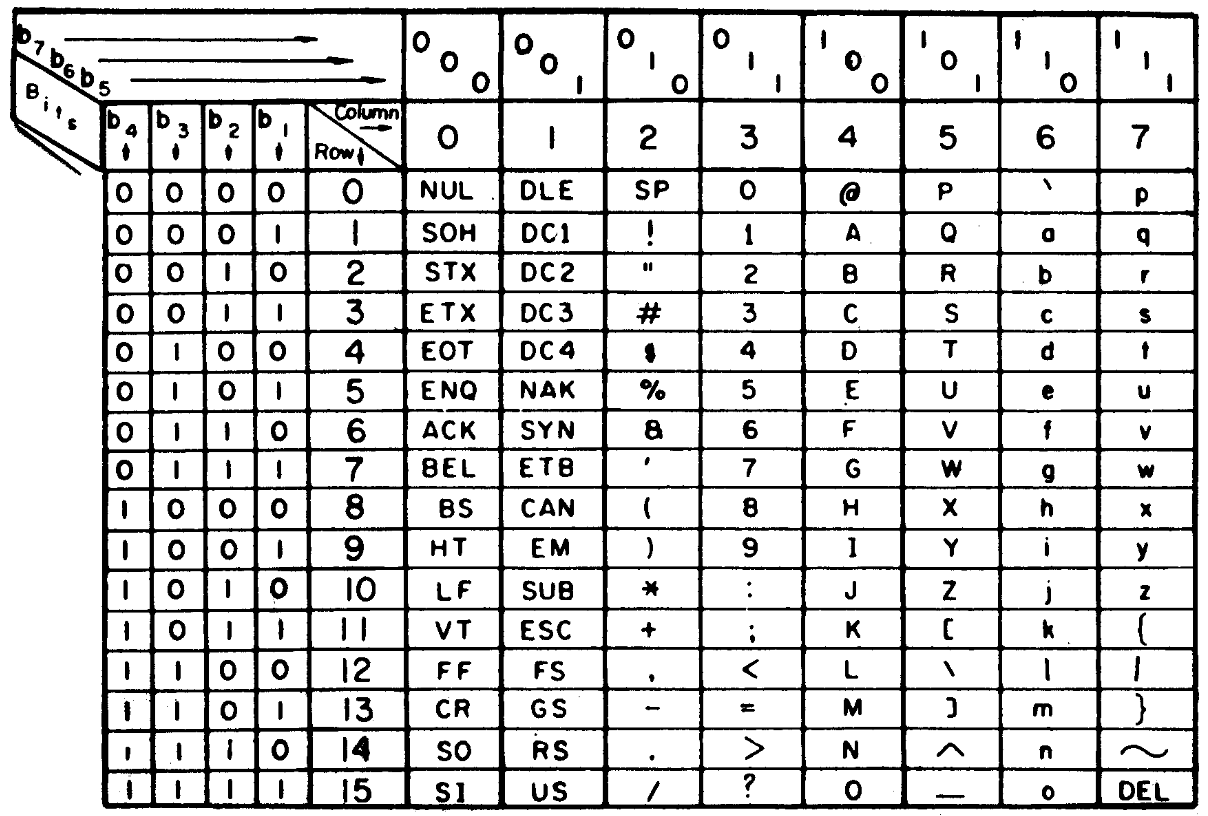
\includegraphics[width=0.75\linewidth]{images/ascii_chart.png}
    \caption{USASCII Code Chart}
\end{figure}
%
\newpage
\subsubsection{Unicode}
Unicode is a modern encoding for many languages and writing systems.
Some characteristics include:
\begin{itemize}
    \item Around 137,000 characters supported
    \item Support for most writing systems
    \item Mathematical symbols, punctuation, emoji
    \item Multiple size encodings
\end{itemize}
Unicode assigns a hexadecimal string (code point) for each character.
It also has several different encodings using different-sized bit strings.
\begin{itemize}
    \item UTF32, using 32 bits for each character
    \item UTF16, using one or two 16-bit strings. This makes it \emph{variable length encoding}
    \item UTF8, using between one and four 8-bit strings.
          It is also \emph{variable length encoding} and is backwards compatible with ASCII.
          UTF8 is the most common encoding
\end{itemize}
%
\subsubsection{Interpreting Text}
Characters are often needed in sequence, forming words.
These are called character strings and are one long string of bits.
Interpreting these bits requires knowing:
\begin{itemize}
    \item How long each character representation is
    \item When to stop
\end{itemize}
For fixed-length encodings, knowing when to stop is sufficient.
Variable-length encodings require a way to recognise when a character representation is finished.
Most modern programming languages store the amount of characters alongside the string.
C however, uses \emph{null-terminated strings} which store a reserved bit string 00000000 (NUL in ASCII)
at the end to indicate the string has ended.

\newpage
\section{Week 3: Propositional Logic}
\subsection{Recursion}
\subsubsection{Recursive Definitions}
An object described in terms of itself is called \emph{recursive definition}.
For example, the factorial of \(\mathbb{N}\) can be defined by:
\[n! = \prod_{j=1}^{n} j = 1 \cdot 2 \dots (n-1) \cdot n\]
\(n!\) can also be defined recursively by:
\[
    n! = 
    \begin{cases}
        1       &: n = 1 \\
        n(n-1)! &: n > 1
    \end{cases}
\]
Another example of recursion is the Fibonacci Sequence:
\[
    f(n) = 
    \begin{cases}
        1               &: n = 1 \\
        1               &: n = 2 \\
        f(n-1) + f(n-2) &: n > 2
    \end{cases}
\]
%
\subsubsection{Recursive Cases}
The two main parts of a recursive definition are:
\begin{itemize}
    \item \textbf{Base cases}: evaluated without any reference to object
    \item \textbf{Recursive cases}: Cases that refer back to object definition
\end{itemize}
At least one base case is required, but there may be several.
Recursive cases must always resolve back to base cases to be well-defined.
\end{document}